\section{\secequivrel}
\label{sec_equiv_relations}

We have seen examples of equivalence in this textbook, including logical equivalence and isomorphic graphs.  You may have seen geometric equivalences such as congruent or similar triangles.  In this section, we formalize the notion of equivalence by defining an equivalence relation and equivalence classes.

%%%%%%%%%%%%%%%%%%%%%%%%

\newcommand{\subrelppty}{Properties of Relations}
\subsection{\subrelppty}
\label{sub_properties_relations}

There are three properties that an relation needs to satisfy in order to be an equivalence relation.

\begin{defn}[Equivalence Relation]
\label{defn_equiv_rel}
    Consider a relation $R$ on a set $X$.
        \begin{apart}
            \item The relation $R$ is \vocab{reflexive} if $(x,x) \in R$ for all $x \in X$.  If the relation is defined by $\sim$, then we need $x \sim x$ for all $x \in X$.  For example, the relation 
                $$R=\{ (a,b) \mid a, b\in \mathbb{Z} \text{ and } ab \ge 0\}$$
            is reflexive on $\mathbb{Z}$, because for any $a \in \mathbb{Z}$ we have $aa=a^2 \ge 0$. Thus $(a,a) \in R$.

            \item The relation $R$ is \vocab{symmetric} if whenever $(x,y) \in R$, then also $(y,x)\in R$ for all $x,y \in X$. If the relation is defined by $\sim$, then we need if $x \sim y$, then $y \sim x$ for all $x,y \in X$.  For example, the relation 
                $$R=\{ (a,b) \mid a, b\in \mathbb{Z} \text{ and } ab = 0\}$$
            is symmetric on $\mathbb{Z}$, because for any $a,b \in \mathbb{Z}$ with $(a,b) \in R$ we have $ab=0$.  Thus $ba=0$ and so $(b,a) \in R$.

            \item The relation $R$ is \vocab{transitive} if whenever $(x,y) \in R$ and $(y,z) \in R$, then $(x,z)\in R$ for all $x,y,z \in X$. If the relation is defined by $\sim$, then we need if $x \sim y$ and $y \sim z$, then $x \sim z$ for all $x,y,z \in X$.  For example, the relation 
                $$R=\{ (a,b) \mid a, b\in \mathbb{Z} \text{ and } a \le b\}$$
            is transitive on $\mathbb{Z}$, because for any $a,b,c \in \mathbb{Z}$ with $(a,b) \in R$ and $(b,c) \in R$ we have $a \le b$ and $b \le c$. Thus $a \le c$ and so $(a,c) \in R$.

            \item The relation $R$ is an \vocab{equivalence relation} if it is reflexive, symmetric, and transitive.  For example, The relation $$R=\{ (a,b) \mid a, b\in \mathbb{Z} \text{ and } a^2=b^2\}$$
            is an equivalence relation.
        \end{apart}
\end{defn}

Let's look at an example of relations on a finite set.

\begin{exam}[Properties of Relations on a Finite Set]
\label{exam_ppty_rel_finite}
    Consider the relation $R$ whose directed graph is drawn in \Cref{fig_rel_finite_ppty}.
        \begin{figure}[hbtp]
            \centering   
            %Used in \Cref{sub_equiv_classes}.

\begin{tikzpicture}[scale =.5,
>=triangle 45,
auto,node distance=1.5cm, thick,
    main node/.style={minimum size=.45 cm, circle,fill=none ,draw}] 
    \node[main node] [label=right:1] (1) {} ; 
    \node[main node] [label=left:2] [below left of=1] (2) {};
    \node[main node] [label=right:3] (3) [below right of =1]{};
    \path[->,
    every loop/.style={min distance=1mm,in=60,out=120,looseness=15}] 
    (1) edge[loop] node { }  (1);
    \path[->,
    every loop/.style={min distance=1mm,in=60,out=120,looseness=20}] 
    (2) edge  node { }    (3);
    \path[->,
    every loop/.style={min distance=1mm,in=60,out=120,looseness=20}] 
    (1) edge  node { }    (3);
    \path[->,
    every loop/.style={min distance=1mm,in=60,out=120,looseness=20}] 
    (2) edge  node { }    (1);
\end{tikzpicture}
%%

            \caption{The relation $R$ is transitive but not reflexive and not symmetric.}
            \label{fig_rel_finite_ppty}
        \end{figure}
        \begin{apart}
            \item Is $R$ reflexive? Justify your answer.
                \begin{soln}
                    No, while there is a loop at 1, there are no loops at 2 or 3.  Thus $(1,1)\in R$, but $(2,2)\notin R$ and $(3,3) \notin R$. To be reflexive, we'd need a loop at every point.
                \end{soln}
            \item Is $R$ symmetric? Justify your answer.
                \begin{soln}
                    No, we have single-headed arrows.  For example, there is an arrow from 2 to 1 but no arrow from 1 to 2.  Thus $(1,2) \in R$, but $(2,1) \in R$.  To be symmetric, we'd need only double-headed arrows and loops.
                \end{soln}
            \item Is $R$ transitive? Justify your answer.
                \begin{soln}
                    Yes.  We need to check if $(x,y) \in R$ and $(y,z) \in R$, then $(x,z) \in R$.  It turns out that there are four $(x,y)$, $(y,z)$ pairs to check as shown in \Cref{tab_rel_finite_trans}.  Since for all four pairs $(x,z) \in R$, the relation is transitive. 

                    \begin{table}[hbtp]
                        \centering
                        \begin{tabular}{llll}
                            $(x,y)$ & $(y,z)$ & $(x,z)$ & in $R$?\\ \hline
                            $(1,1)$ & $(1,1)$ & $(1,1)$ & Yes\\
                            $(1,1)$ & $(1,3)$ & $(1,3)$ & Yes\\
                            $(2,1)$ & $(1,1)$ & $(2,1)$ & Yes\\
                            $(2,1)$ & $(1,3)$ & $(2,3)$ & Yes\\
                        \end{tabular}
                        \caption{Justifying that the relation $R$ drawn in \Cref{fig_rel_finite_ppty} is transitive.}
                        \label{tab_rel_finite_trans}
                    \end{table}
                \end{soln}
        \end{apart}
\end{exam}

Your turn to work with properties of relations

\begin{act}[Properties of relations]
\label{act_ppty_rel}

    For parts (\ref{part_act_rel_ppty_reflexive})-(\ref{part_act_rel_ppty_not_trans}), consider the relations on $X = \{1,2,3\}$ defined by $T = \{(1,1),(1,2), (2,2), (2,3),(3,1),(3,3)\}$ and $V =  \{(1,1), (2,3), (3,2)\}$. \Cref{fig_TandV} shows their directed graph.
        \begin{figure}[hbtp]
            \centering
            %Used in \Cref{sec_equiv_relations}.

\begin{tikzpicture}[scale =.5,
>=triangle 45,
auto,node distance=1.5cm, thick,
    main node/.style={minimum size=.45 cm, circle,fill=none ,draw}] 
    \node at (0,4) {$T$};
    \node[main node] [label=right:1] (1) {} ; 
    \node[main node] [label=left:2] [below left of=1] (2) {};
    \node[main node] [label=right:3] (3) [below right of =1]{};
        \path[->,
    every loop/.style={min distance=1mm,in=60,out=120,looseness=20}] 
    (1) edge  node { }    (2);
        \path[->,
    every loop/.style={min distance=1mm,in=60,out=120,looseness=20}] 
    (2) edge  node { }    (3);
    \path[->,
    every loop/.style={min distance=1mm,in=60,out=120,looseness=20}] 
    (3) edge  node { }    (1);
        \path[->,
    every loop/.style={min distance=1mm,in=60,out=120,looseness=15}] 
    (1) edge[loop] node { }  (1);
        \path[->,
    every loop/.style={min distance=1mm,in=-60,out=-120,looseness=15}] 
    (2) edge[loop] node { }  (2);
        \path[->,
    every loop/.style={min distance=1mm,in=-60,out=-120,looseness=15}] 
    (3) edge[loop] node { }  (3);
\end{tikzpicture}
\hspace{1in} %%%%%
\begin{tikzpicture}[scale =.5,
>=triangle 45,
auto,node distance=1.5cm, thick,
    main node/.style={minimum size=.45 cm, circle,fill=none ,draw}]
    \node at (0,4) {$V$};
        \node at (0,-4.5) {}; % To raise V
    \node[main node] [label=right:1] (1) {} ; 
    \node[main node] [label=left:2] [below left of=1] (2) {};
    \node[main node] [label=right:3] (3) [below right of =1]{};
    \path[->,
    every loop/.style={min distance=1mm,in=60,out=120,looseness=15}] 
    (1) edge[loop] node { }  (1);
    \path[<->,
    every loop/.style={min distance=1mm,in=60,out=120,looseness=20}] 
    (2) edge  node { }    (3);
\end{tikzpicture}

            \caption{The relations $T$ and $V$ from \Cref{act_ppty_rel}.}
            \label{fig_TandV}
        \end{figure}
        \begin{actpart}
            \item \label{part_act_rel_ppty_reflexive} Give a counterexample to show that $V$ is not reflexive.  Is $T$ reflexive?  Explain.
            \item Give a counterexample to show that $T$ is not symmetric.  Is $V$ symmetric?  Explain.
            \item Give a counterexample to show that $T$ is not transitive.
            \item \label{part_act_rel_ppty_not_trans}Give a counterexample to show that $V$ is not transitive. Hint: The values of $x$, $y$, and $z$ do not need to be distinct.
            \item Consider the relation on $\mathbb{Z}$ defined by $$\{(a,b) \mid a, b \in \mathbb{Z} \text{ and }\fn{gcd}(a,b)=1\}.$$  Decide which properties $R$ has: reflexive, symmetric, transitive.  No justification is required if the relation has the property, but provide a counterexample if not.
            \item Consider the relation $\sim$ on $\mathbb{R}^2$ defined by $(x_1,y_1) \sim (x_2,y_2)$ if $y_2-y_1=3(x_2-x_1)$.  Check that $\sim$ is an equivalence relation.  Hint: For transitive, note that $(y_3-y_2)+(y_2-y_1)=y_3-y_1.$
        \end{actpart}
\end{act}

Each of the relations $T$ and $V$ in \Cref{act_ppty_rel} was not transitive, but for fundamentally different reasons. Let's take a closer look at transitivity of relations on a finite set.

\begin{exam}[When is a relation on finite set transitive?]
\label{exam_rel_finite_not_trans}
    We saw in \Cref{exam_ppty_rel_finite} how to use the directed graph of a relation on a finite set to determine whether the relation is reflexive or symmetric.  How can we use the directed graph of a relation on a finite set to determine whether the relation is transitive? 
        \begin{soln}
            Suppose $R$ is a relation on a finite set $X$ and that  $(x,y) \in R$ and $(y,z) \in R$.
            There are four cases, as drawn in \Cref{fig_shortcuts_barbells}.  
                \begin{figure}[hbtp]
                    \centering
                    %Used in \Cref{sec_equiv_relations}.

\begin{tikzpicture}[scale =.5,
>=triangle 45,
auto,node distance=1.5cm, thick,
    main node/.style={minimum size=.45 cm, circle,fill=none ,draw}] 
    \node at (0,3.5) {$x$, $y$, $z$ distinct};
    \node at (0,2.5){shortcut};
    \node[main node] [label=above:$x$]  (x) {} ; 
    \node[main node] [label=below:$y$] [below left of=1] (y) {};
    \node[main node]  [label=below:$z$] (z) [below right of =1]{};
        \path[->,
    every loop/.style={min distance=1mm,in=60,out=120,looseness=20}] 
    (x) edge  node { }    (y);
        \path[->,
    every loop/.style={min distance=1mm,in=60,out=120,looseness=20}] 
    (y) edge  node { }    (z);
        \path[dashed,->,
    every loop/.style={min distance=1mm,in=60,out=120,looseness=20}] 
    (x) edge  node { }    (z);
\end{tikzpicture}
\hspace{.1in} %%%%%
\begin{tikzpicture}[scale =.5,
>=triangle 45,
auto,node distance=1.5cm, thick,
    main node/.style={minimum size=.45 cm, circle,fill=none ,draw}] 
    \node at (0,3.5) {$x=y$};
    \node at (0,2.5){always true/ignore};
    \node[main node] [label=below:$x$] [below left of=1] (x) {};
    \node[main node]  [label=below:$z$] (c) [below right of =1]{};
        \path[->,
    every loop/.style={min distance=1mm,in=60,out=120,looseness=20}] 
    (x) edge  node { }    (z);
        \path[ ->,
    every loop/.style={min distance=1mm,in=60,out=120,looseness=15}] 
    (x) edge[loop] node { }  (x);
\end{tikzpicture}
\hspace{.1in} %%%%%
\begin{tikzpicture}[scale =.5,
>=triangle 45,
auto,node distance=1.5cm, thick,
    main node/.style={minimum size=.45 cm, circle,fill=none ,draw}] 
    \node at (0,3.5) {$y=z$};
    \node at (0,2.5){always true/ignore};
    \node[main node] [label=below:$x$] [below left of=1] (x) {};
    \node[main node]  [label=below:$z$] (c) [below right of =1]{};
        \path[->,
    every loop/.style={min distance=1mm,in=60,out=120,looseness=20}]
    (x) edge  node { }    (z);
        \path[ ->,
    every loop/.style={min distance=1mm,in=60,out=120,looseness=15}] 
    (z) edge[loop] node { }  (z);
\end{tikzpicture}
\hspace{.1in} %%%%%
\begin{tikzpicture}[scale =.45,
>=triangle 45,
auto,node distance=1.5cm, thick,
    main node/.style={minimum size=.45 cm, circle,fill=none ,draw}] 
    \node at (0,3.8) {$x=z\neq y$};
    \node at (0,2.8){barbells};
    \node[main node] [label=below:$x$] [below left of=1] (x) {};
    \node[main node]  [label=below:$y$] (y) [below right of =1]{};
        \path[<->,
    every loop/.style={min distance=1mm,in=60,out=120,looseness=20}]
    (x) edge  node { }    (y);
        \path[dashed, ->,
    every loop/.style={min distance=1mm,in=60,out=120,looseness=15}] 
    (x) edge[loop] node { }  (x);
        \path[dashed, ->,
    every loop/.style={min distance=1mm,in=60,out=120,looseness=15}] 
    (y) edge[loop] node { }  (y);
\end{tikzpicture}
                    \caption{Shortcuts and barbells: checking transitivity on finite relation.}
                    \label{fig_shortcuts_barbells}
                \end{figure}

            Case 1: First, consider when $x$, $y$, and $z$ are three distinct elements of $X$.  Then the directed graph has arrows from $x$ to $y$ and from $y$ to $z$. We need to check if $(x,z) \in R$, indicated by the dashed arrow from $x$ to $z$ in our diagram.  To be transitive, any time we have a two-step path in the directed graph, we must also have the \vocab{shortcut (vector sum)}.

            Case 2: Next, consider when $x=y$ or $y=z$. If $x=y$, then $(x,z) =(y,z)\in R$.  If $y=z$, then $(x,z) =(x,y)\in R$. In either case $(x,z)$ is automatically in $R$ so we can ignore this case.

            Case 3: The remaining case is when $x = z$. We need to check $(x,x)=(x,z) \in R$.  Swapping order, we also need to check $(z,z)=(z,x)\in R$. That is, any time there is a double-headed arrow in the graph, we need to have a loop at each end, or \vocab{barbells}, which we draw in our diagram with dashed loops. 
        \end{soln}
\end{exam}

Equivalence relations can be defined on all types of discrete objects.

\begin{exam}[Examples of equivalence relations on graphs]
\label{exam_equiv_rel_graphs}
    Consider the set $G_6$, the set of all graphs on six vertices.  Give some examples of equivalence relations on $G_6$.
        \begin{soln}
            There are many different examples. Here are a few:
                \begin{itemize}
                    \item $G \sim H$ if $G$ and $H$ have the same number of edges.  
                    \item $G \sim H$ if $G$ and $H$ have the same degree sequence.
                    \item $G \sim H$ if $G$ and $H$ contain the same number of 3-cycles. 
                    \item $G \sim H$ if $G \cong H$, where $\cong$ denotes that the graphs are isomorphic.
                \end{itemize}
        \end{soln}
\end{exam}

%%%%%%%%%%%%%%%%%%%%%%%%

\newcommand{\subequivclass}{Equivalence Relations and Equivalence Classes}
\subsection{\subequivclass}
\label{sub_equiv_classes}

An important construction in advanced theoretical mathematics is to take a set $X$ and an equivalence relation $\sim$ on $X$ and define a new set consisting of the equivalence classes of $X$ under $R$.  We begin with the definitions.

\begin{defn}[Equivalence classes]
\label{defn_equiv_class}
    Consider a set $X$ and an equivalence relation $R$ (or $\sim$) on $X$.
        \begin{apart}
            \item For any element $a \in X$, the \vocab{equivalence class containing} $a$ is the set 
                $$[a]=\{b \in X \mid (a,b) \in R\} = \{b \in X \mid a \sim b\}.$$
            For example, for the relation $$R=\{ (a,b) \mid a, b\in \mathbb{Z} \text{ and } a^2 =b^2 \},$$
            the equivalence class of $3$ is $[3] = \{3,-3\}$.  Note that $[-3]=\{3,-3\}$ is the same set.

            \item The \vocab{quotient space}, denoted $X/R$ and pronounced ``$X$ mod $R$'', is the set of all equivalence classes.  For example, for the relation $R = \{(a,b) \mid a, b\in \mathbb{Z} \text{ and } a+b \text{ is even}\},$
            there are two equivalence classes: $[0]=$ the even integers and $[1]=$ the odd integers.  Thus $\mathbb{Z}/R = \{[0],[1]\}$.  
        \end{apart}
\end{defn}

Let's look at an example.

\begin{exam}[Equivalence classes for an equivalence relation on $\{1,2,3,4,5\}$]
\label{exam_equiv_classes_12345}
    Consider the equivalence relation $R$ on $X = \{1,2,3,4,5\}$ defined by the directed graph drawn in \Cref{fig_equiv_rel_12345}.
        \begin{figure}[hbtp]
            \centering
            %Used in \Cref{sec_equiv_relations}.

\begin{tikzpicture}[scale =.35,
    >=triangle 45,auto,node distance=1.5cm, thick] 
\GraphInit[vstyle=Welsh]
\SetGraphUnit{1.6}
    %%%% Vertices
        \Vertex[LabelOut,Lpos=180,x=0,y=6]{1}
        \Vertex[LabelOut,Lpos=90,x=4,y=3]{2}
        \Vertex[LabelOut,Lpos=45,x=2,y=0]{3}
        \Vertex[LabelOut,Lpos=135,x=-2,y=0]{4}
        \Vertex[LabelOut,Lpos=90,x=-4,y=3]{5}
    %%%% Loops at each point
        \path[->, every loop/.style={min distance=1mm,in=60,out=120,looseness=15}] 
            (1) edge[loop] node { }  (1);
        \path[->, every loop/.style={min distance=1mm,in=-30,out=30,looseness=15}] 
            (2) edge[loop] node { }  (2);
        \path[->, every loop/.style={min distance=1mm,in=-60,out=0,looseness=15}] 
            (3) edge[loop] node { }  (3);
        \path[->, every loop/.style={min distance=1mm,in=180,out=240,looseness=15}] 
            (4) edge[loop] node { }  (4);
        \path[->, every loop/.style={min distance=1mm,in=150,out=210,looseness=15}] 
            (5) edge[loop] node { }  (5);
    %%%% Additional double-headed arrows
        \path[<->] (2) edge  node { }    (5);
        \path[<->] (1) edge  node { }    (3);
        \path[<->] (3) edge  node { }    (4);
        \path[<->] (4) edge  node { }    (1);
\end{tikzpicture}

            \caption{An equivalence relation on $\{1,2,3,4,5\}$.}
            \label{fig_equiv_rel_12345}
        \end{figure}
        \begin{apart}
            \item Calculate $[1]$.
                \begin{soln}
                    There are three arrows out of 1 or, equivalently, three ordered pairs of the form $(1,\underline{\quad~})$, namely $(1,1)$, $(1,3)$, and $(1,4)$.  Thus $[1]=\{1,3,4\}$.
                \end{soln}
            \item Calculate $[2]$.
                \begin{soln}
                    There are two arrows out of 2 or, equivalently, two ordered pairs of the form $(2,\underline{\quad~})$, namely $(2,2)$ and $(2,5)$.  Thus $[2]=\{2,5\}$.
                \end{soln}    
            \item How many different equivalence classes are there?
                \begin{soln}
                    We can check that $[3]=\{1,3,4\}$, $[4]=\{1,3,4\}$, and $[5]=\{2,5\}$.  Therefore, there are only two equivalence classes:  $\{1,3,4\}$ and $\{2,5\}$. It is convenient to refer to these equivalence classes using the smallest possible representative as $[1]$ and $[2]$. 
                \end{soln}
            \item Describe the quotient space $X/R$.
                \begin{soln}
                    The quotient space consists of two equivalence classes:  $X/R=\{[1],[2]\}$.  
                \end{soln}
        \end{apart}
\end{exam}

Try working with equivalence classes.

\begin{act}[Equivalence classes]
\label{act_equiv_classes}
~
    \begin{actpart}
        \item Consider the relation $R$ on $\{1,2,3,4\}$ defined by $R= \{(1,1),(1,2),(2,1),(2,2),(3,3),(4,4)\}$.  Identify the equivalence classes $[1]$, $[2]$, $[3]$, and $[4]$.  How many distinct equivalence classes are there?
        
        \item \label{part_equiv_rel_given_partition} Draw the directed graph of the equivalence relation on $\{1,2,3,4,5,6\}$ with equivalence classes $\{1,2,3\}$, $\{4\}$, and $\{5,6\}$.
        
        \item Consider the equivalence relation $R$ on $\mathbb{Z}$ defined by
            $$R=\{ (a,b) \mid a, b\in \mathbb{Z} \text{ and } a^2 =b^2 \}.$$
        Calculate $[2]$, $[-4]$, and $[0]$.
        
        \item Consider the equivalence relation $\sim$ on $\mathbb{R}^2$ defined by $(x_1,y_1) \sim (x_2,y_2)$ if  $y_2-y_1=3(x_2-x_1)$.  Describe the equivalence class $[(0,2)]$.

        \item \label{part_bs5_start_same3} Let $\mathbb{B}_5$ be the set of all bit strings of length 5.  Consider the equivalence relation on $\mathbb{B}_5$ defined by $b \sim c$ if the bit strings $b$ and $c$ start with the same three bits.  For example, $\bs{11111} \sim \bs{11100}$ and $\bs{10111} \sim \bs{10110}$.  Calculate $[11111]$ and $[10111]$.  

        \item Continuing with the relation $\sim$ on $\mathbb{B}_5$ defined in (\ref{part_bs5_start_same3}). How many (distinct) equivalence classes are there and how many bit strings are in each equivalence class?

        \item Give an example of an equivalence relation on $\mathbb{B}_5$, the bit strings of length 5, that has exactly two equivalence classes.  Now give a different one.
    \end{actpart}
\end{act}

In \Cref{exam_equiv_classes_12345}, we had an equivalence relation on the set $\{1,2,3,4,5\}$ and the equivalence classes were $\{1,3,4\}$ and $\{2,5\}$.  Note that $\{1,3,4\} \cup \{2,5\}$ is a partition of the set $\{1,2,3,4,5\}$, as defined in \Cref{defn_partition}.  Conversely, in \Cref{act_equiv_classes} (\ref{part_equiv_rel_given_partition}, we had a partition $\{1,2,3\} \cup \{4\} \cup \{5,6\}$ of the set $\{1,2,3,4,5,6\}$ and we determined the directed graph of an equivalence relation $R$ on $\{1,2,3,4,5,6\}$ having those subsets as equivalence classes. This connection between equivalence classes and partitions of a set holds in general.

\begin{rem}[Equivalence classes and partitions]
\label{rem_equiv_class_partition}
    Let $X$ be a set.  
        \begin{apart}
            \item If $R$ is an equivalence relation on $X$, then the distinct equivalence classes under $R$ form a partition of the set $X$.
            \item If $T_1 \cup T_2 \cup \cdots \cup T_k$ is a partition of $X$, then the relation on $R$ defined by $(x,y) \in R$ if $x$ and $y$ are both in the same set $T_i$ for some $i$ is an equivalence relation. Moreover, its equivalence classes are exactly $T_1, T_2, \ldots, T_k$.
        \end{apart}
\end{rem}

%%%%%%%%%%%%%%%%%%%%%%%%

\newcommand{\subcongmod}{Congruence mod $n$}
\subsection{\subcongmod}
\label{sub_cong_modn}

An important equivalence relation on $\mathbb{Z}$ is defined using $\fn{mod}$. 

\begin{defn}[Congruence mod $n$]
\label{defn_cong_modn}
~
    \begin{apart}
        \item For a positive integer $n$, the integers $a$ and $b$ \vocab{are congruent modulo} $n$, denoted $a \equiv b ~(\fn{mod} ~n)$, if $a \fn{~mod~} n = b \fn{~mod~} n$, that is, if $a$ and $b$ have the same remainder when divided by $n$.  For example, $73 \equiv 13 ~(\fn{mod} ~10)$ because $73 \fn{~mod~} 10 = 3$ and $73 \fn{~mod~} 10 = 3$.  As another example, for any integer $a$, if $a ~\fn{mod}~ n=r$, then  that $a \equiv r ~(\fn{mod} ~n)$.  For example, $73 \equiv 3 ~(\fn{mod} ~10)$.  It turns out that congruence modulo $n$ is an equivalence relation.
        
        \item For a positive integer $n$, the \vocab{congruence class mod $n$} of $a$ is 
            $$[a]_n = \{ b \in \mathbb{Z} \mid a \equiv b ~(\fn{mod} ~n)\}.$$  
        Note that the congruence class is the equivalence class under the congruence relation.
        For example, 
            $$[3]_{10} = \{\ldots, -17, -7, 3, 13, 23, 33, 43, \ldots\}.$$
        \item The \vocab{integers mod} $n$ introduced in \Cref{sec_mod_arith} is formally defined as $$\mathbb{Z}_n = \{[0]_n, [1]_n, \ldots, [n-1]_n\}.$$  For example, $\mathbb{Z}_3 = \{[0]_3, [1]_3, [2]_3\}$.
    \end{apart}
\end{defn}

Note that if $a \fn{ mod } n = b \fn{ mod } n$, then $a$ and $b$ end at the same number on the $\fn{mod } n$ clock.  Therefore, $a$ and $b$ differ by some number of complete rotations, which is multiple of $n$.  We have the following result.

\begin{thm}[Alternate characterization of congruence \fn{mod} $n$]
\label{thm_cong_modn}
    Let $a$, $b$, and $n$ be integers with $n > 1$.  Then $a \equiv b ~(\fn{mod } n)$ if and only if $n | (a-b)$.
\end{thm}

Let's look at some examples.

\begin{exam}[Using the alternate characterization of congruence \fn{mod} $n$]
\label{exam_alt_defn_cong}
~
    \begin{apart}
        \item Use \Cref{thm_cong_modn} to show that $73 \equiv 13 ~(\fn{mod } 10)$.
            \begin{soln}
                We can check that $73-13 = 60 = 10(6)$ and so $10 \mid (73-13)$. Thus $73 \equiv 13 ~(\fn{mod } 10)$.
            \end{soln}
        \item \label{part_proof_cong} Prove that if $a \equiv b ~(\fn{mod } n)$, then $2a \equiv 2b ~(\fn{mod } n)$ for any integers $a$, $b$, and $n$ with $n > 1$.
            \begin{soln}
                Since we are proving a conditional statement, we use \Cref{pff_if_then_direct}.

                \emph{Proof} Let $a$, $b$, and $n$ be integers with $n > 1$. Assume $a \equiv b ~(\fn{mod } n)$.  By \Cref{thm_cong_modn}, it follows that $n \mid (a-b)$.  By \Cref{defn_divides}, we can write $a-b = nk$ for some integer $k$.  Then
                $$ 2a - 2b = 2(a-b) = 2(nk) = n(2k) = nk'$$
                where $k' = 2k$ is an integer.  By \Cref{defn_divides}, it follows that $n \mid (2a-2b).$  By \Cref{thm_cong_modn}, it follows that $2a \equiv 2b ~(\fn{mod } n)$.
            \end{soln}
        \item State the converse of the statement from (\ref{part_proof_cong}) and construct a counterexample to show that the converse is false. 
            \begin{soln}
                The converse is: if $2a \equiv 2b ~(\fn{mod } n)$, then $a \equiv b ~(\fn{mod } n)$ for any integers $a$, $b$, and $n$ with $n > 1$.  For a counterexample we need integers $a$, $b$, and $n$ with $n > 1$ such that the promise is broken.  That is, we want $2a \equiv 2b ~(\fn{mod } n)$ but $a \not\equiv b ~(\fn{mod } n)$. A counterexample is $a=2$ and $b=7$ because $4 \equiv 14 ~(\fn{mod } 10)$ but $2 \not\equiv 7 ~(\fn{mod } 10)$.
            \end{soln}
    \end{apart}
\end{exam}

Try working with congruence mod $n$.

\begin{act}[Congruence \fn{mod} $n$]
\label{act_cong_modn}  
~
    \begin{actpart}
        \item  True or false?  $73 \equiv 13 ~(\fn{mod } 2)$
        \item  True or false?  $73 \equiv 13 ~(\fn{mod } 3)$
        \item  True or false?  $73 \equiv 13 ~(\fn{mod } 4)$
        \item  True or false?  $73 \equiv 13 ~(\fn{mod } 5)$
        \item  Find a counterexample to the statement $73 \equiv 13 ~(\fn{mod } n)$ for all integers $n >1$.  Hint: $73-13=60$.
        \item Describe the integers in $[0]_2$.
        \item Describe the integers in $[0]_3$.
        \item How many congruence classes are there \fn{mod} 10?  Explain.
        \item Explain why congruence \fn{mod} $n$ is reflexive, symmetric, and transitive.
    \end{actpart}
\end{act}

%%%%%%%%%%%%%%%%%%%%%%%%

\subsection{Exercises}

%%%%%%%%%%%%%%%%%%%%%%%%

\subsubsection*{Exercises for \Cref{sub_properties_relations}
\subrelppty}

\begin{exer}[\exerP] % counterexamples for relation on $\mathbb{Z}$]
\label{exer_Cex_rel_on_integers}
~
    \begin{exerpart}
        \item Construct a counterexample to show the relation $\{ (a,b) \mid a, b  \in \mathbb{Z} \text{ and } a < b \}$ is not reflexive.
        \item Construct a counterexample to show the relation $\{ (a,b) \mid a, b  \in \mathbb{Z}^+ \text{ and } a \mid b \}$ is not symmetric. 
        \item Construct a counterexample to show the relation $\{ (a,b) \mid a, b  \in \mathbb{Z} \text{ and } ab = 0 \}$ is is not transitive.
    \end{exerpart}
\end{exer}

\begin{exer}[\exerP] % counterexamples for relation on $\mathbb{R}$]
\label{exer_Cex_rel_on_reals}
~
    \begin{exerpart}
        \item Construct a counterexample to show the relation $\{ (x,y) \mid x, y  \in \mathbb{R} \text{ and } x + y = 5 \}$ is not reflexive.
        \item Construct a counterexample to show the relation $\{ (x,y) \mid x, y  \in \mathbb{R} \text{ and } x \ge y \}$ is not symmetric.
        \item Construct a counterexample to show the relation $\{ (x,y) \mid x, y  \in \mathbb{R} \text{ and } |x - y | < 3 \}$ is not transitive.
    \end{exerpart}
\end{exer}

\begin{exer}[\exerP] % transitivity of finite relations]
\label{exer_finite_rel_transitive}
~
    \begin{exerpart}  
        \item Construct a counterexample to show that the relation $\{(0,0), (0,1), (1,1), (1,2), (2,0), (2,2)\}$ is not transitive.
        \item Construct a counterexample to show that the relation $\{(0,0), (0,1), (1,0), (2,2)\}$ is not transitive.
        \item Show how to check that the relation $\{(0,0), (0,1), (1,1), (1,2), (0,2), (2,2)\}$ is transitive.  Note: It is okay to not check loops.
    \end{exerpart}
\end{exer}

\begin{exer}[\exerU] % properties finite relations]
\label{exer_ppty_finite_rel}
    For each relation, draw the directed graph on $\{0,1,2\}$ and then decide if the relation is reflexive, symmetric, and transitive.  For each part, no justification required if the relation has the property, but provide counterexample if not.
        \begin{exerpart}
            \item $\{(0,0), (0,1), (1,0), (1,1), (1,2), (2,2)\}$
            \item $\{(0,0), (0,1), (0,2), (1,1), (1,2), (2,2)\}$ % partial order
            \item $\{(0,0), (0,1), (1,0), (1,1), (2,2)\}$ % equivalence relation
        \end{exerpart}
\end{exer}

\begin{exer}[\exerU] % relations on \{0,1\}]  
\label{exer_ppty_rel01}
    On this problem, no justification is required.
        \begin{exerpart}
            \item Draw the directed graph for each relation on $\{0,1\}$ that is reflexive.
            \item \label{part_01_sym_and_refl} Draw the directed graph for each relation on $\{0,1\}$ that is symmetric and reflexive.
            \item \label{part_01_not_trans} Draw the directed graph for each relation on $\{0,1\}$ that \emph{not} transitive. Hint: Barbells
            \item Draw the directed graph for each equivalence relations on $\{0,1\}$.  Hint: Use your lists from (\ref{part_01_sym_and_refl}) and (\ref{part_01_not_trans}).
        \end{exerpart}
\end{exer}

\begin{exer}[\exerU] % properties empty and complete relation]
\label{exer_name_empty_complete_rel}
    Let $X$ be a nonempty set.  For each relation, decide whether it is reflexive, whether it is symmetric, and whether it is transitive.  No justification required if the relation has the property, but provide counterexample if not.
        \begin{exerpart}
            \item The relation $\varnothing$ 
            \item The relation $X^2$ % equiv
        \end{exerpart}
\end{exer}

\begin{exer}[\exerU] % decide properties relations on $\mathbb{Z}^+$]
\label{exer_ppty_rel_on_integers}
    For each relation, decide whether it is reflexive, whether it is symmetric, and whether it is transitive. No justification required if relation has the property, but provide counterexample if not. 
        \begin{exerpart}
            \item $\{(a,b) \mid a,b \in \mathbb{Z}^+ \text{ and } ab \text{ is even}  \}$
            \item $\{(a,b) \mid a,b \in \mathbb{Z}^+ \text{ and }  ab \text{ is odd} \}$
            \item $\{(a,b) \mid a,b \in \mathbb{Z}^+ \text{ and }  \fn{gcd}(a,b)\neq1~ \}$
            As usual, $\fn{gcd}$ denotes the greatest common divisor, as defined in \Cref{defn_gcd}.
        \end{exerpart}
\end{exer}

\begin{exer}[\exerU] % decide properties unit circle]
\label{exer_ppty_rel_unit_circle}
    Consider the unit circle 
        $$U=\{(x,y) \mid x, y \in \mathbb{R} \text{ and } x^2+y^2=1\}$$
    which is drawn in \Cref{fig_unit_circle_verticallinetest}.  For each part, no justification is required if $U$ has the property, but provide counterexample if not. 
        \begin{exerpart}
            \item Is $U$ reflexive?
            \item Is $U$ symmetric?
            \item Is $U$ transitive?
        \end{exerpart}
\end{exer}

\begin{exer}[\exerU] % property distance at most 5 relation]
\label{exer_ppty_distance_le5}
    Consider the relation defined on $\mathbb{R}^2$ by $(x_1,y_1) \sim (x_2,y_2)$ if $$\sqrt{(x_1-x_2)^2 + (y_1-y_2)^2} \le 5.$$
        \begin{exerpart}
            \item Is $(1,2) \sim (1,7)$? Explain.
            \item Is $(1,2) \sim (5,0)$? Explain.
            \item Is $\sim$ reflexive?  Explain.
            \item Construct a counterexample to show that $\sim$ is not transitive.
        \end{exerpart}
\end{exer}

\begin{exer}[\exerU] % properties relation on bit strings]
\label{exer_ppty_rel_bs}
   For each relation, decide whether it is transitive.  Explain briefly if it is transitive and construct a counterexample if not transitive.
    \begin{exerpart}
        \item As usual $\mathbb{B}^*$ denotes the set of all (non-empty) bit strings. Define a relation on $\mathbb{B}^*$ by $b \sim c$ if $b$ is a \textbf{substring} of $c$; that is, if the bit string $b$ appears in consecutive order within the bit string $c$.  For example, $\bs{101} \sim \bs{111010}$ as we can see $\bs{11}\underline{\bs{101}}\bs{0}$. 
        \item Consider the set $\mathbb{B}_3$, the set of all bit strings of length 3.  Define the relation $b \sim c$ if the bit strings $b$ and $c$ differ in exactly one bit.  For example, $100 \sim 110$ and $100 \sim 000$.
    \end{exerpart}
\end{exer}

\begin{exer}[\exerU] % properties relations on power set]
\label{exer_ppty_rel_power_set}
    Consider the following relations on $\mathscr{P}(\{1,2,3\})$.        
        \begin{exerpart}
            \item Give a counterexample to show that $\{(A,B) \mid ~ A \cup B = S ~ \}$ is not reflexive. 
            \item Give a counterexample to show that $\{(A,B) \mid ~ A \subseteq B~ \}$ is not symmetric.
            \item Give a counterexample to show that $\{(A,B) \mid ~ A \cap B = \varnothing ~ \}$ is not transitive.
        \end{exerpart}
\end{exer}

\begin{exer}[\exerU] % same size finite sets]
\label{exer_prove_same_size_set_equiv_rel}
    For the set $\mathscr{P}(\{1,2,3, \ldots, n\})$, define $A \sim B$ if $|A| = |B|$ (meaning $A$ and $B$ have the same number of elements). Check that $\sim$ is an equivalence relation.  Show how to check each property in general.
\end{exer}

\begin{exer}[\exerR] % properties of relations
\label{exer_dyk_ppty_rel}
    Do you know \ldots
        \begin{exerpart}
            \item How to decide if a relation is reflexive, symmetric, or transitive?
            \item How to construct a counterexample to show that a relation is not reflexive, not symmetric, or not transitive?
        \end{exerpart}
\end{exer}

\begin{exer}[\exerE] % definition antisymmetric]
\label{exer_defn_antisym}
    A relation $R$ on a set $X$ is \vocab{antisymmetric} if whenever $(x,y) \in R$ with $x \neq y$ we have $(y,x) \notin R$. No justification required if "yes", but provide counterexample if "no". 
        \begin{exerpart}
            \item Is the relation R on $\{(0,0), (0,1), (1,0), (2,2)\}$ antisymmetric? 
            \item Is the relation $\{(0,0), (0,1), (1,1), (1,2), (0,2), (2,2)\}$ antisymmetric? 
            \item Is the relation $\{ (a,b) \mid a, b  \in \mathbb{Z} \text{ and } a < b \}$  antisymmetric? 
            \item Is the relation $\{ (a,b) \mid a, b  \in \mathbb{Z}^+ \text{ and } a \mid b \}$  antisymmetric? As usual, $\mid$ denotes divides, as defined in \Cref{defn_divides}.
        \end{exerpart}
\end{exer}

\begin{exer}[\exerE] % symmetric vs. antisymmetric]
\label{exer_ppty_rel_sym_vs_antisym}
    In \Cref{exer_defn_antisym} we defined antisymmetric. In each part, give an example of a relation on $\{0,1,2,3\}$ meeting the conditions. No justification required.
        \begin{exerpart}
            \item Antisymmetric and not symmetric.
            \item Symmetric and not antisymmetric.
            \item Neither symmetric nor antisymmetric.
            \item Both symmetric and antisymmetric.
        \end{exerpart}
\end{exer}

\begin{exer}[\exerE] % definition partial order]
\label{exer_defn_partial_order}
    A relation $R$ on a set $X$ is a \vocab{partial order} if $R$ is reflexive, antisymmetric, and transitive. Prove that the relation $\{ (x,y) \mid x, y  \in \mathbb{R} \text{ and } x \le y \}$ is a partial order on $\mathbb{R}$.      
    (By the way, some other examples of partial orders are $\le$ or $\ge$ on any sets of real numbers, $\mid$ (divides) on the positive integers, $\subseteq$ on the power set of any set, and contains as a substring on the set of all (non-empty) bit strings, as in \Cref{exer_ppty_rel_bs}.)
\end{exer}

%%%%%%%%%%%%%%%%%%%%%%%%

\subsubsection*{Exercises for \Cref{sub_equiv_classes}
\subequivclass}

\begin{exer}[\exerP] % equivalence classes on $\{1,2,3,4,5,6,7\}$]
\label{exer_equiv_classes_1234567}
    Consider the equivalence relation on $\{1,2,3,4,5,6,7\}$ defined by 
        $$R=\{(1,1), (1,2), (1,5), (2,1), (2,2), (2,5), (3,3),(3,4),$$
        $$ (4,3), (4,4), (5,1), (5,2), (5,5), (6,6), (6,7), (7,6), (7,7)\}.$$
\begin{exerpart}
    \item Calculate $[5]$.
    \item Calculate $[6]$.
    \item How many distinct equivalence classes are there? Explain briefly.
    \item Draw the directed graph of a new equivalence relation on $\{1,2,3,4,5,6,7\}$ with exactly two distinct equivalence classes:  $\{1,2,3,4\}$ and $\{5,6,7\}$.
\end{exerpart}    
\end{exer}

\begin{exer}[\exerP] % equivalence classes involving the floor function]
\label{exer_equiv_classes_floor}
    For each equivalence relation on $\mathbb{R}^+$ (the positive real numbers), describe the equivalence class [7.3].  Hint: If you are  not sure where to start, find examples of real numbers $y$ such that $7.3 \sim y$.
        \begin{exerpart}
            \item \label{part_integer_part} The equivalence relation defined by $x \sim y$ if $\lfloor x \rfloor = \lfloor y \rfloor$. 
            \item \label{part_fractional_part} The equivalence relation defined by $x \sim y$ if $x-\lfloor x \rfloor = y-\lfloor y \rfloor$.
            \item Restate the relation from (\ref{part_integer_part}) in the form ``$x \sim y$ if $x$ and $y$ have the same $\underline{\hspace{1in}}$.  Repeat for the relation from (\ref{part_fractional_part}). 
        \end{exerpart}   
\end{exer}

\begin{exer}[\exerP] % equivalence relation on $\mathbb{R}^2$]
\label{exer_equiv_classes_slope3}
    Consider the equivalence relation defined on $\mathbb{R}^2$ by $(x_1,y_1) \sim (x_2,y_2)$ if  $y_2-y_1=3(x_2-x_1)$ that we saw in \Cref{sec_relations} \Cref{exer_slope_relation}.
        \begin{exerpart}
            \item Describe $[(0,0)]$.
            \item Describe $[(1,0)]$.
            \item In general, describe each equivalence class.  Hint: It is a set in the $xy$-plane.
        \end{exerpart}
\end{exer}

\begin{exer}[\exerP] % first coordinate equivalence relation on $\mathbb{R}^2$]
\label{exer_equiv_classes_first_coord}
    Consider the equivalence relation defined on $\mathbb{R}^2$ by $(x_1,y_1) \sim (x_2,y_2)$ if  $x_1=x_2$
        \begin{exerpart}
            \item Describe $[(0,0)]$.
            \item Describe $[(1,0)]$.
            \item In general, describe each equivalence class. Hint: It is a set in the $xy$-plane.
        \end{exerpart}
\end{exer}

\begin{exer}[\exerU] % all equivalence classes on small finite sets]
\label{exer_all_equiv_classes_small_finite}
~
    \begin{exerpart}
        \item Draw the directed graphs for both equivalence relation on $X = \{1,2\}$ and list the equivalence classes for each.
        \item Repeat for $X = \{1,2,3\}$.  Hint: There are five different equivalence relations.
        \item How many different equivalence relations are there on $X = \{1,2,3,4\}$?  Explain your count.
    \end{exerpart}
\end{exer}

\begin{exer}[\exerU] % equality as an equivalence relation]
\label{exer_equiv_rel_equality}
~  
    \begin{exerpart}
        \item  For any set $X$, \vocab{equality} $E = \{(x,y) \mid x=y\}$ is the smallest possible equivalence relation.If $X$ is finite, what does the directed graph of $E$ look like?  Describe the equivalence classes of $E$.
        \item At the other extreme,  $X^2$ itself is an equivalence relation on $X$.  If $X$ is finite, what does the directed graph of  $X^2$ look like? How many equivalence classes are there?
    \end{exerpart}
\end{exer}

\begin{exer}[\exerU] % same weight bit strings]
\label{exer_bs_equiv_same_weight}
    Consider the set $\mathbb{B}_5$, the set of all bit strings of length 5.  Define the equivalence relation on $\mathbb{B}_5$ by $b \sim c$ if the bit strings $b$ and $c$ have the same weight, that is if $b$ and $c$ have the same number of \bs{1}s.  For example, $\bs{00111} \sim \bs{11010}$ and only $\bs{11111} \sim \bs{11111}$.
        \begin{exerpart}
            \item Calculate $[\bs{00111}]$ and $[\bs{11111}]$.  
            \item How many (distinct) equivalence classes are there?
            \item For each equivalence class, state how many bit strings are in that equivalence class.
        \end{exerpart}
\end{exer}

\begin{exer}[\exerU] % equivalence classes of bit strings that start with the same two bits]
\label{exer_bs_equiv_same_2bits}
    Consider the set $\mathbb{B}_5$, the set of all bit strings of length 5.  Define the equivalence relation $b \sim c$ if the bit strings $b$ and $c$ start with the same two bits.  For example, $11111 \sim 11000$ and $10111 \sim 10101$.
        \begin{exerpart}
            \item Calculate $[11111]$ and $[10111]$.  
            \item How many (distinct) equivalence classes are there?
            \item How many bit strings are in each equivalence class?
        \end{exerpart}
\end{exer}

\begin{exer}[\exerU] % same size sets]
\label{exer_equiv_classes_same_size_sets}
    For $\mathscr{P}(\{1,2,3,4,5\})$, we saw in \Cref{exer_prove_same_size_set_equiv_rel} that the relation $A \sim B$ if $|A| = |B|$, meaning that $A$ and $B$ have the same number of elements, is an equivalence relation.
        \begin{exerpart}
            \item Calculate $[\{1,3\}]$ and [$\phi$].
            \item How many (distinct) equivalence classes are there?
            \item For each equivalence class, state how many subsets are in that equivalence class. 
            \item Comment on how this exercise relates to \Cref{exer_bs_equiv_same_weight}.
        \end{exerpart}
\end{exer}

\begin{exer}[\exerU] % equivalence classes defined by functions]
\label{exer_equiv_classes_fns}
    For any set $X$ and any function $f:X \to X$, the relation on $X$ defined by  $x_1 \sim x_2$ if $f(x_1) = f(x_2)$ is always an equivalence relation.   
        \begin{exerpart} 
            \item For readers who are familiar with trigonometry, describe $[0]$ where $f: \mathbb{R} \to \mathbb{R}$ is defined by $f(x) = \fn{sin}(x)$.
            \item For the function $f: \mathbb{Z} \to \mathbb{Z}$ defined by $f(n) = n^2$, explain why the equivalence classes are $$\{0\}, \{1,-1\}, \{2,-2\}, \{3,-3\}, \{4,-4\}, \ldots$$  Now give two more examples of functions with the same equivalence classes.
            \item What can we say about a function $f$ if each equivalence class is a \vocab{singleton} (one element set)?
        \end{exerpart} 
\end{exer}

\begin{exer}[\exerU] % same 2-part]
\label{exer_equiv_classes_2part}
    Define an equivalence relation on $\mathbb{Z}$ by $a \sim b$ if $a$ and $b$ have the same 2-part, that is, $a \sim b$ if $a = 2^km$ and $b=2^kn$ for some nonnegative integer $k$ and odd integers $m$ and $n$.
        \begin{exerpart}
            \item Verify that $12 \sim 20$.
            \item Verify that $35 \sim 11$.
            \item Describe the equivalence class $[1]$.
            \item Describe the equivalence class $[2]$.
        \end{exerpart}
\end{exer}

\begin{exer}[\exerU] % defining the rational numbers]
\label{exer_equiv_classes_rationals}
    Define the equivalence relation on $\mathbb{Z} \times\mathbb{Z}^\ast$ by $(a_1,b_1) \sim (a_2,b_2)$ if $a_1b_2 = a_2b_1$.  By the way, the rational numbers $\mathbb{Q}$ is the quotient space $\mathbb{Z}/\sim$.
        \begin{exerpart}
            \item Verify that $(4,6) \sim (2,3)$.  
            \item Describe the equivalence class $[(2,3)]$.  
        \end{exerpart}
\end{exer}

\begin{exer}[\exerR] % equiv relns
\label{exer_dyk_equiv_rel}
    Do you know \ldots
        \begin{exerpart}
            \item What three properties a relation needs to satisfy in order to be an equivalence relation?
            \item How to find the equivalence class of an element under a relation?
            \item What we mean by ``distinct'' equivalence classes?
            \item What the connection is between equivalence classes and partitions of a set?
        \end{exerpart}
\end{exer}

\begin{exer}[\exerE] % $2 \times 2$ gray-and-white grids]
\label{exer_2x2_GW-grids}
    Consider the set $X$ consisting of all $2 \times 2$ grids where each of the four smaller squares is colored either gray or white.  An example is drawn in \Cref{fig_2x2_GW_grid}.
        \begin{figure}[hbtp]
            \centering
            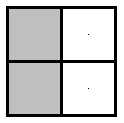
\includegraphics[width=0.1\linewidth]{Images/2x2_gray_and_white.png}
            \caption{An example of a $2 \times 2$ gray-and-white grid for \Cref{exer_2x2_GW-grids}.}
            \label{fig_2x2_GW_grid}
        \end{figure}
        \begin{exerpart}
            \item How many different $2 \times 2$ grids are there?  Note that any number of the squares can be gray or white, not necessarily two of each as shown.
            \item For grids $G$ and $H$, define an equivalence relation on $X$ by $G \sim H$ if we can rotate $G$ to obtain $H$.  Calculate $[G]$ where $G$ is the square drawn in \Cref{fig_2x2_GW_grid}. 
            \item Under $\sim$, how many different equivalence classes of $2 \times 2$ grids are there?  Draw one $2 \times 2$ grid from each equivalence class.
        \end{exerpart}
\end{exer}

\begin{exer}[\exerE] % equivalence classes defined by the derivative]
\label{exer_equiv_class_derivative}
    For readers who have studied calculus, consider the set $X$ of all differentiable functions $f: \mathbb{R} \to \mathbb{R}$.  Define an equivalence relation on $X$ by $f \sim g$ if $f' = g'$, meaning $f'(x) = g'(x)$ for all $x \in \mathbb{R}$.  That is, two functions are equivalent if they have the same derivative function.
        \begin{exerpart}
            \item Describe $[f]$ where $f: \mathbb{R} \to \mathbb{R}$ is defined by $f(x) = 3x+1$.
            \item Describe $[g]$ where $g: \mathbb{R} \to \mathbb{R}$ is defined by $g(x) = xe^x$. Hint: you do not need to know what $g'(x)$ is, just which functions have the same derivative as $g$.
        \end{exerpart} 
\end{exer}

%%%%%%%%%%%%%%%%%%%%%%%%

\subsubsection*{Exercises for \Cref{sub_cong_modn}
\subcongmod}

\begin{exer}[\exerP] % definition of congruence mod $n$]
\label{exer_check_congruent_modn}
    Briefly justify your answers.
        \begin{exerpart}
            \item Is $70 \equiv 34 ~(\fn{mod }5)$?
            \item Is $70 \equiv 34 ~(\fn{mod }6)$?
            \item  Is $70 \equiv 34 ~(\fn{mod }11)$?
        \end{exerpart}
\end{exer}

\begin{exer}[\exerU] % Converses and Cex congruences
\label{exer_converse_cex_cong_modn}
    State the converse (\Cref{defn_converse}) of each statement and then prove that the converse is false by constructing a counterexample. Each statement refers to all integers $a$, $b$, and $n$ with $n>1$.  
        \begin{exerpart}
            \item If $a \equiv b ~(\fn{mod }n)$, then $3a \equiv 3b\text{ (mod }n)$.
            \item If $a \equiv b \text{ (mod }n)$, then $a^2 \equiv b^2\text{ (mod }n)$.  
            \item If $a \equiv 0 ~(\fn{mod }n)$ or $b \equiv 0 ~(\fn{mod }n)$, then $ab \equiv 0 ~(\fn{mod }n)$.
        \end{exerpart}
\end{exer}

\begin{exer}[\exerU] % proof congruences
\label{exer_proof_cong_modn}
    Let $a$, $b$, and $n$ be integers with $n>1$.  Prove each of the following statements using \Cref{thm_cong_modn}.  Hint: Copy and edit the proof in \Cref{exam_alt_defn_cong} (\ref{part_proof_cong}) . 
        \begin{exerpart}
            \item If $a \equiv b ~(\fn{mod }n)$, then $3a \equiv 3b\text{ (mod }n)$.
            \item If $a \equiv b \text{ (mod }n)$, then $a+2 \equiv b+2\text{ (mod }n)$.
            \item If $a \equiv b \text{ (mod }n)$, then $a^2 \equiv b^2\text{ (mod }n)$.  Hint: $a^2-b^2=(a+b)(a-b)$.
        \end{exerpart}
\end{exer}

\begin{exer}[\exerR] % cong mod n
\label{exer_dyk_cong_modn}
    Do you know \ldots
        \begin{exerpart}
            \item What $a \equiv b ~(\fn{mod}~n)$ means?
            \item How to prove statements involving congruences?
            \item How to find counterexamples to false statements involving congruences?
            \item How the congruence class \fn{mod} $n$ is defined?
        \end{exerpart}
\end{exer}

%%%%%%%%%%%%%%%%%%%%%%%%%%%
\subsection{\answers}
%%%%%%%%%%%%%%%%%%%%%%%%%%%

%%%%%%%%%%%%%%%%%%
\subsubsection{\answers for \Cref{sub_properties_relations}
\subrelppty}

\subsubsection*{\Cref{exer_Cex_rel_on_integers} \answers}
\begin{apart}
    \item Hint: One possible counterexample is $(5,5)$ because $5<5$ is false.  Provide a different counterexample.
    \item Hint: Find integers $a$ and $b$ where $a \mid b$ but $b \nmid a$.
    \item Hint: Use one of $a$ or $b$ equal to 0. 
\end{apart}

\subsubsection*{\Cref{exer_Cex_rel_on_reals} \answers}
\begin{apart}
    \item Hint: One possible counterexample is $(2,2)$ because $2+2 \neq 5$.
    \item Hint: Find real numbers $x$ and $y$ with $x \ge y$ but not $y \ge x$.
    \item Hint: Try some examples.
\end{apart}

\subsubsection*{\Cref{exer_finite_rel_transitive} \answers}
\begin{apart}
    \item Hint: Find a missing shortcut.
    \item Hint: Barbells
    \item Hint: For example, check $(0,1)$ and $(1,2)$ are in the relation and $(0,2)$ is too.
\end{apart}

\subsubsection*{\Cref{exer_ppty_finite_rel} \answers}
\begin{apart}
    \item Hint: It is reflexive, but not symmetric and not transitive.
    \item Hint: It has two of the three properties.
    \item Hint: It is an equivalence relation.
\end{apart}

\subsubsection*{\Cref{exer_ppty_rel_on_integers} \answers}
\begin{apart}
    \item Hint: It is not reflexive and not transitive.
    \item Hint: The only way $ab$ is odd is if $a$ is odd and $b$ is odd.
    \item Hint: It is not reflexive but there's only one possible counterexample.
\end{apart}

\subsubsection*{\Cref{exer_ppty_distance_le5} \answers}
\begin{apart}
    \item Hint: Yes
    \item Hint: No
    \item Hint: Yes
    \item Hint: Try using $(0,0)$ as the second ordered pair to construct a counterexample.
\end{apart}

\subsubsection*{\Cref{exer_ppty_rel_bs} \answers}
\begin{apart}
    \item Hint: It is transitive.
    \item Hint: It is not transitive.
\end{apart}

\subsubsection*{\Cref{exer_ppty_rel_power_set} \answers}
Recall that $\mathscr{P}(\{1,2,3\})$ is the power set of $\{1,2,3\}$, the set of all subsets of $\{1,2,3\}$.
\begin{apart}
    \item Hint: One counterexample is $(\{1,2\},\{1,2\})$.
    \item Hint: Find subsets $A$ and $B$ where $A \subseteq B$ but not $B \subseteq A$.
    \item Hint: Start with subsets $A$ and $B$ such that $A \cap B = \varnothing$.  Then try to find a set $C$ with $B \cap C = \varnothing$ but $A \cap C \neq \varnothing$.
\end{apart}

%%%%%%%%%%%%%%%%%%
\subsubsection{\answers for \Cref{sub_equiv_classes}
\subequivclass}

\subsubsection*{\Cref{exer_equiv_classes_1234567} \answers}
\begin{apart}
    \item $\{1,2,5\}$
    \item Hint: There are two elements in $[6]$.
    \item Hint: Calculate $[3]$.  Then count the distinct ones.
    \item Hint: Make sure you have included all the necessary loops and double-headed arrows.
\end{apart}

\subsubsection*{\Cref{exer_equiv_classes_slope3} \answers}
\begin{apart}
    \item It is the line $y = 3x$ which has slope 3 and $y$-intercept 0.
    \item Hint: It is a different line.
    \item Hint: What do the lines have in common?
\end{apart}

\subsubsection*{\Cref{exer_equiv_classes_first_coord} \answers}
\begin{apart}
    \item It is the line $x=0$ which is the $y$-axis.
     \item Hint: It is a different line.
     \item Hint: What do the lines have in common?
\end{apart}

\subsubsection*{\Cref{exer_bs_equiv_same_weight} \answers}
\begin{apart}
    \item Hint: There are ten bit strings in $[\bs{00111}]$ but only one bit string in $[\bs{11111}]$.
    \item Hint: The answer is not five.
    \item Hint: Different classes may contain different number of bit strings.
\end{apart}

\subsubsection*{\Cref{exer_bs_equiv_same_2bits} \answers}
\begin{apart}
    \item Hint: $[\bs{11111}] = \{\bs{11000}, \bs{11001}, \ldots, \bs{11111}\}$ and $[\bs{10111}]$ contains the same number of bit strings.
    \item Four
    \item Hint: They each contain the same number of bit strings.
\end{apart}

\subsubsection*{\Cref{exer_2x2_GW-grids} \answers}
\begin{apart}
    \item Hint: Count using steps with Step 1 is deciding if the upper left-hand corner is gray or white.  Then continue with each of the four squares.
    \item Hint: There are four squares in $[G]$, one of which is $G$ itself.
    \item Hint: Draw one $2 \times 2$ grid from each equivalence class, being sure that no two grids you draw are equivalent.  Then count how many grids you drew.
\end{apart}

%%%%%%%%%%%%%%%%%%
\subsubsection{\answers for \Cref{sub_cong_modn}
\subcongmod}

\subsubsection*{\Cref{exer_check_congruent_modn} \answers}
Hint: Two answers are no.

\subsubsection*{\Cref{exer_converse_cex_cong_modn} \answers}
\begin{apart}
    \item Hint: Make $n$ a multiple of 3.
    \item Hint: Try $n=10$ because \fn{mod} 10 is easy to compute (just the last digit)
    \item Hint: Try $n=10$ again.
\end{apart}
